\documentclass[a4paper,12pt]{article} % ce document est un article sur une feuille A4, police taille 12

\usepackage[utf8]{inputenc} % encodé en utf-8
\usepackage[T1]{fontenc} % compatible avec les accents

\usepackage[round]{natbib} % gestion des citations
\usepackage[french]{babel} % rédigé en français
\usepackage[hyphens]{url} % formatte les liens en autorisant la césure au niveau des traits d'union
\usepackage[pdftex,urlcolor=black,colorlinks=true,linkcolor=black,citecolor=black]{hyperref} % liens cliquables mais non colorés
\usepackage[top=3cm,bottom=4cm]{geometry} % gère les marges
\usepackage{graphicx} % gestion des images
\usepackage{array} % gestion des tableaux
\usepackage{csquotes} % gestion des guillemets
\usepackage{fourier} % utilise une autre police que celle par défaut (Computer Modern)
\usepackage{setspace}% gestion des interlignes
\onehalfspacing
% insérez ici d'autres extensions avec la commande \usepackage[options]{nom de l'extension}

\title{QUEL LANGAGE DE PROGRAMMATION CHOISIR POUR CREER UN LOGICIEL ?} % le titre de l'article
\author{Abdel Josselin POUAMOUN} % vos prénom et nom
\date{} % pas de date

\begin{document} % début du corps du texte
\maketitle % affiche le titre

\section{INTRODUCTION} % section 1
Un ordinateur est une machine électronique programmable servant au traitement de l'information. Il peut être  assimilé à un système produisant des résultats à partir : d'informations fournies , et de méthode de résolution permettant de traiter ces informations.
Les informations constituent des données et les méthodes de résolution aident à construire des algorithmes qui représentent l'enchaînement des actions à réaliser qui sont nécessaires à la résolution d'un problème donné et dont la traduction dans un langage de programmation permet de réaliser un programme, une application ou un logiciel.
Lorsque nait l’idée de conception d’un projet logiciel, la première question qu’on devrait se poser, c’est de savoir avec quel langage de programmation  on doit le développer ? 
C’est bien beau de vouloir programmer ou d’apprendre un langage de programmation, mais il faut savoir lequel choisir, et pour cela un ensemble de  critère devrait être examiné au préalable.
Écrire des programmes nécessite l'utilisation d'un langage de programmation (ou plusieurs). Il y a toute une pléthore de langages de programmation disponibles. Ces langages ne sont pas, forcement équivalents bien qu’il existe parfois certaines similitudes entre eux. Chaque langage possède ses avantages et ses inconvénients.
Faisons ainsi un tour des questions à se poser (critères à examiner) pour choisir correctement son langage de programmation.
Afin de choisir un langage ou une implémentation, un programmeur doit tenir compte d'un certain nombre paramètres :
\begin{itemize}
\item[$\bullet$]L’utilisabilité du langage
Facilité d'apprentissage, et facilité d'utilisation pour un programmeur expérimenté.
\item[$\bullet$]Les performances du langage
Rapidité d'exécution des programmes, rapidité d'exécution du compilateur,  stabilité (absence de défaut)…
\item[$\bullet$]La portabilité du langage sur différentes plateformes
Sa capacité à pouvoir être adapté plus ou moins facilement en vue de fonctionner dans différents environnements d'exécution. Les différences peuvent porter sur l'environnement matériel (processeur) comme sur l'environnement logiciel (système d'exploitation).
\item[$\bullet$]L’extensibilité du langage
Perspectives d'évolution du langage ou de son implémentation, existence de bibliothèques de fonctions, de classes, etc.,
\item[$\bullet$]La pérennité du langage
Pérennité du fabricant, pérennité du langage, pérennité de l'implémentation, existence d'une norme internationale concernant la définition du langage. Conformité de l'implémentation par rapport à la norme, existence de plusieurs fabricants pour le même langage.
\item[$\bullet$]La documentation du langage
\end{itemize}
Connaître un langage de programmation est un atout de plus en plus important sur le marché du travail, puisque la demande de développeurs de logiciels augmente de façon exponentielle ces dernières années.
Cependant, quand on débute dans la programmation, on peut être confus face aux centaines de langages que l’on peut choisir. C’est pour cela que je rédige cet article afin de conseiller les futurs programmeurs dans le choix du langage idéal pour eux.
  % Contenu de l'introduction

\section{Qu’est-ce qu’un langage de programmation ?} % section 2
Un langage de programmation est un langage permettant de formuler des algorithmes et de produire des programmes informatiques qui appliquent ces algorithmes.

Un programme est un enchaînement d'instruction, écrit dans un langage de programmation, exécutée par un ordinateur, permettant de traiter un problème et de renvoyer des résultats. Il représente la traduction un algorithme à l'aide d'un langage de programmation.
\begin{figure}[h] % insère une figure ici (h = "here")
  \centering % centre la figure
  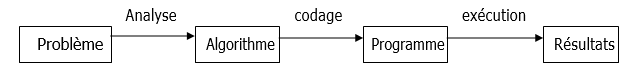
\includegraphics[scale=1]{img1.PNG} % insère une image en taille réelle
\end{figure}
L'ordinateur est une machine totalement dénuée d'intelligence. Un programme exécute les instructions bien précises c'est-à-dire celle que le programmeur lui a donnée. Des erreurs ou des fantaisies lors de son exécution ne proviennent pas de l'ordinateur mais d'une erreur de conception.

\section{Evolution des langages de programmation} % section 3

Un ordinateur ne connaît que le système de numération binaire. Un langage utilisant le système binaire s'appelle langage machine.
Pour écrire des programmes sous des formes accessibles,les langages d'assemblage ont vu le jour au début des années 50, 
 
Cependant, un programme écrit en langage d'assemblage n'est pas directement exécutable par la machine. Il doit être traduit en un programme équivalent en langage machine. Cette opération de traduction s'effectue grâce à un autre programme appelé assembleur.
Le langage d'assemblage présente un inconvénient : il reste lié à l'ordinateur pour lequel il a été écrit car chaque famille de processeurs possède son propre langage d'assemblage. Il est difficile à utiliser car il nécessite de bonnes connaissances sur le fonctionnement des processeurs.
C'est pourquoi furent conçus les langages de programmation dits évolués plus compréhensibles et plus lisibles par l'homme.
Un langage de programmation est défini par des règles d'écriture des règles de construction que doivent respecter les programmes. La difficulté, pour le programmeur, consiste à respecter ses règles imposées en fonction des differents paradigmes de programmation.


\end{document} % fin du corps du texte